\chapter{Conclusions and Recommendations for Further Work}

\section{Summary and Main Conclusions}

Following the review of literature which is located in (Chapter 3), four main research questions were identified regarding the project as a whole.

\begin{enumerate}
    \item\textbf{\textit{Is there a need for an application like this on the marketplace?}}
    
    \item\textbf{\textit{Is there a way to save battery life while using GPS / Internet connection within an android application?}}
    
    \item\textbf{\textit{Will location services, and mobile internet take much battery or data?}} 
    
    \item\textbf{\textit{Will the APP provide a wiki type interface where visitors can add to the information about a historic site?}}
    
\end{enumerate}  

\subsection{Developments and Findings Relating to Research Objective 1}  
With regards to the following question on which the author is to provide an answer to is yes there is quite a market for this application. The developer of InforMe@Dublin has received many words of praise before even releasing an app of the following standard. Researching application's of this type and standard throughout the Google Play market are of non-existence the developer of which had released a small survey to the general public of Lucan as a pilot scheme on distinguishing if the idea of an application within its category would fit in with their need's. Utilising a survey website called Survey Monkey was used in the creation of the survey which was published to the people of Lucan.

\begin{figure}[htbp]
    \center 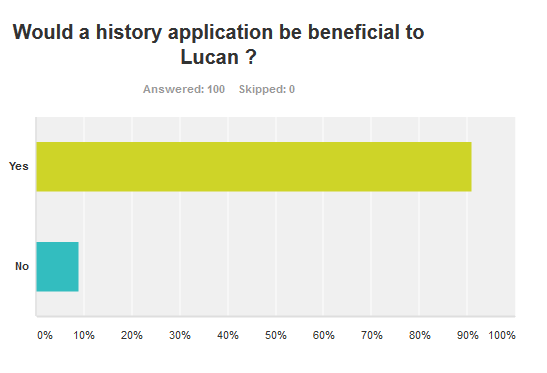
\includegraphics[width=350pt]{Lucan}\\
    \caption{Need for InforMe@Dublin} \label{Figure: Need for InforMe@Dublin}
\end{figure}

Regarding figure 9.1 the developer has shown one of the results on which were retrieved from the survey of which suggests that the people of Lucan would love to see an application of the following stature.

\begin{figure}[htbp]
    \center 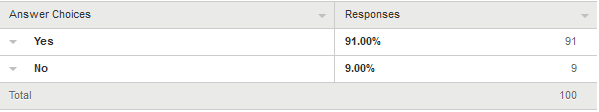
\includegraphics[width=350pt]{Lucanresponces}\\
    \caption{Number of Patrons who Completed Survey} \label{Figure: Number of Patrons who Completed Survey}
\end{figure}

The number of patrons who took part in the survey with relation to seeing if the InforMe@Dublin application was a good choice. 91 out of the 100 patrons who completed the survey said that they would be interested in such an application while nine said no. This could be that some of the patrons who took part in the survey were not actually from Dublin and may live in other area's or that the specific audience of which was targeted wasn't the best choice such as 15 - 19 year old's.

An application which is related to the InforMe@Dublin that the developer has found was produced for the telling of information of the 1916 rising located here in Dublin City Centre the app of which was developed by Failte Ireland. The Dublin Discovery Trails application is for the use of guided tours within the city centre itself which tells the story of Dublin over 1000 years. The app which use's devices location but stores all necessary files on the application itself and is only useful in Dublin city before going on these walks the application prompts user's to download a specific audio and image files which isn't much use if the patron is on the go.

\subsection{Developments and Findings Relating to Research Objective 2}
Regarding objective two which is related to the life of a battery while using location services as well as the internet connectivity. The battery life can be saved by using Google Play Services of which provide a battery manager of which is provided within the application to provide the best and most suitable power/accuracy ratio on gaining the location of an Android device.

The answer is yes. The battery life of an Android phone can be optimised by being smart with the development of the application. Breaking each part into specific smaller piece’s allowing threads to do individual tasks will help the life of the user’s battery, Also by using less service’s such as not calling all of the Google service’s packages will assist the battery life by using only a particular package. \cite{andBatt}

As the following application is to be used for educational purposes and doesn't ambit the need for adverts of which provides 75\% of application related battery drain. The following study was provided by Purdue University in partnership with Microsoft. These studies were concluded by looking at free application's located in the Google Play Store and the Apple store. As ad-serving provides its advertisers with valuable data from many patrons of many applications. In a nutshell advertiser's cover the cost of the application which is why it is delivered free to the user. The problem of these Ad-serving SDK's are that they are in fact poorly coded with regards to sending the information back to servers as well as the activity on the screen.\cite{admob} 

Also while using Firebase on which is incorporated within the Android application allows for the saving of some data on which has been loaded from the database this allows for the device to show this data which doesn't need to be parsed and downloaded again.

\subsection{Developments and Findings Relating to Research Objective 3}
While retrieving the location of a mobile device the following information was retrieved from a source which provides each of the location techniques, as well as the amount of power each of these, utilise while in use. This information was gathered when the author was researching different technologies that would be used or potentially used in the application.
\begin{table}[!ht]
    \centering
    \caption{Battery Usage of Positioning Techniques \cite{bareth2011energy}}
    \label{Battery Usage of Positioning Techniques}
    \begin{tabular}{@{}llrl@{}}
        \toprule
        \multicolumn{1}{c}{\textit{Technologies}} & \textit{Accuracy} & \textit{Precision} & \textit{Energy} \\ \midrule
        GPS & 10m & 95\% & 6.616Ws \\ \midrule
        WiFi & 50m & 90\% & 2.852Ws \\ \midrule
        Cellular-ID & 5km & 65\% & 1.013Ws \\ \bottomrule
    \end{tabular}
\end{table}

The following screen shot located in figure 9.3 was taken from the test device of which the InforMe@Dublin application was developed on. In the figure below shows how much data of which the application had consumed over the hour test. Below shows that on average the application does not exactly use that much data compared to other applications over an hour interval.

\begin{figure}[htbp]
    \center 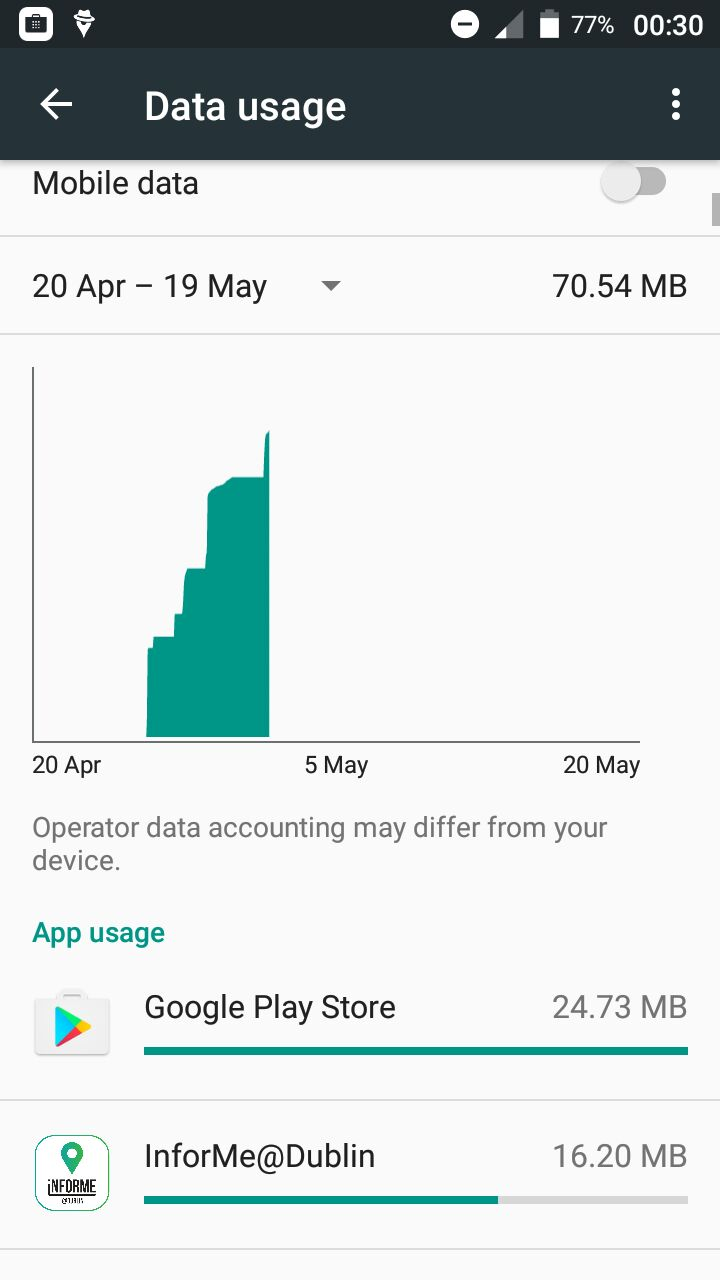
\includegraphics[width=150pt]{dataused}\\
    \caption{Data usage of InforMe@Dublin} \label{Figure: Data usage of InforMe@Dublin}
\end{figure}
\newpage

\subsection{Developments and Findings Relating to Research Objective 4}
During the development of such an application, the developer decided on introducing a different type Wiki feel to the application which allows the users to contribute to the information on such areas by posting different images of that area whether that being new or old images. While each patron has added their individual information of the area. Other users can then like posts of which have been created. Only that specific user who created the post can remove and update it on the application if they wish to re-visit the Geofence location. A Screen-shot of the applications wiki type feel is shown below in figure - 9.4

\begin{figure}[htbp]
    \center 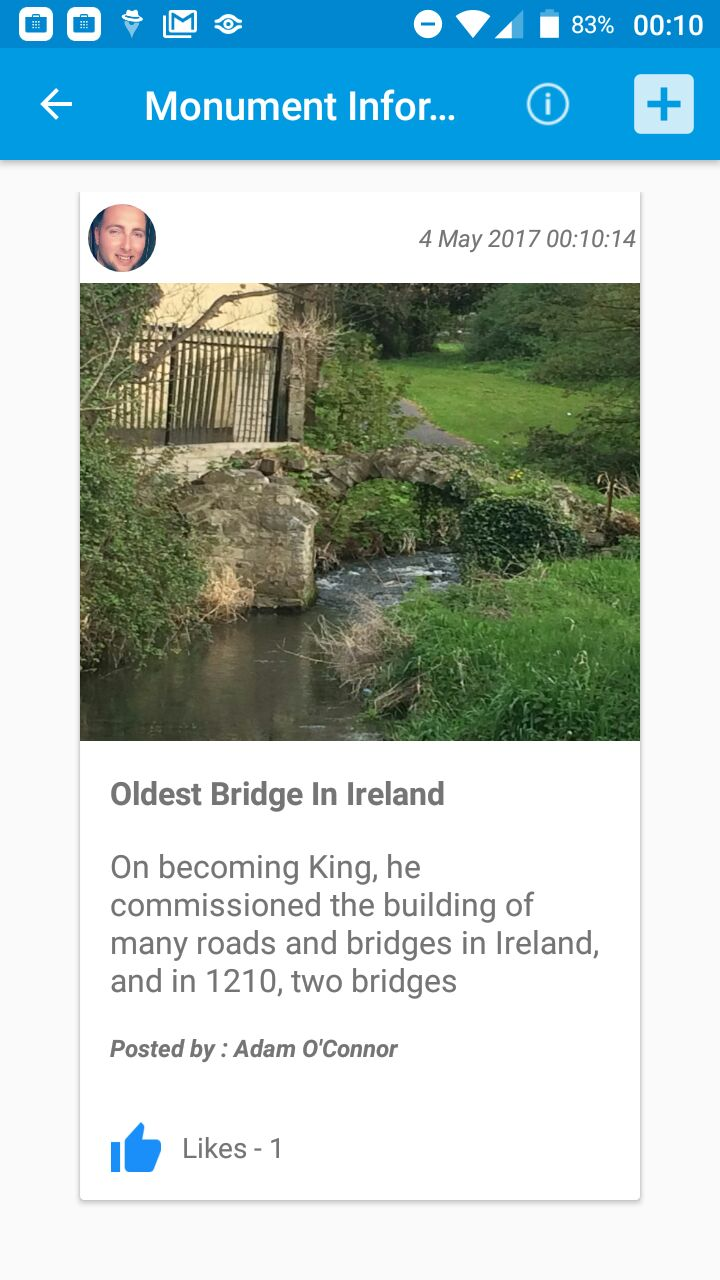
\includegraphics[width=150pt]{wikifeel}\\
    \caption{Wiki Type Activity} \label{Figure: Wiki Type Activity}
\end{figure}
\newpage

\section{Recommendations for Further Work}
With regards to the developer continuing with the development of the Android application InforMe@Dublin. The developer as follows thinks that the project as a whole is worthy of more development bringing the app to even more devices as it is only limited to Android Marshmallow devices and above. With the future of technology where it is today, there is a significant opportunity for providing an application to other users not just specifically to Dublin so the Informe app can be expanded and provided to people all over Ireland.

the following future work objectives can be completed.
\begin{enumerate}
    \item Providing more historical monuments to the application.
    \item Adding a new way of users to add a Geofence.
    \item Creation of specific profile pages of user's.
    \item Providing more cost effective ways on users using the application with a connection to the internet.
    \item Provide more power efficient code which allows users to explore more.
    \item Adding a how to page or tutorial on how to use the InforMe@Dublin application.
\end{enumerate}
